% Plantilla común para figuras redibujadas (fig-NN-desc.tex).
% Copiar entera y sustituir solo el cuerpo entre las marcas "cuerpo de la figura".
% Compila tal cual en Overleaf o con scripts/tikz2svg.sh.
%
% NO añadir la opción "tikz" a standalone: parte cada tikzpicture (y cada
% \chemfig) en una página distinta y el SVG solo tendría la primera.
\documentclass[border=4pt]{standalone}
\usepackage[T1]{fontenc}
\usepackage{lmodern}            % base vectorial: sin fuente vectorial el texto sale en Type 3 y dvisvgm lo pierde
\usepackage[scaled=0.95]{helvet}% sans-serif tipo Helvetica, como la interfaz de Obsidian
\renewcommand{\familydefault}{\sfdefault}
\usepackage{amsmath,amssymb}
\usepackage{sansmath}\sansmath  % fórmulas en sans, a juego con el texto
\usepackage[version=4]{mhchem}  % \ce{A + B -> C}
\usepackage{chemfig}            % estructuras y esquemas de reacción
\usepackage{tikz}
\usetikzlibrary{arrows.meta,positioning,calc,shapes.geometric,decorations.pathmorphing,decorations.markings}
\usepackage{pgfplots}           % gráficas (cinética, curvas de valoración...)
\pgfplotsset{compat=1.18}

% ---- Estilo Apuntes.md --------------------------------------------------
% Paleta semántica (la misma que el CSS de Obsidian). Principios inspirados en
% figures4papers (ChenLiu-1996, CC BY-NC 4.0): se adoptan ideas, no código.
\definecolor{apAzul}{HTML}{0F4D92}       % anotaciones, estructura (el azul del autor)
\definecolor{apAzulClaro}{HTML}{3775BA}
\definecolor{apRojo}{HTML}{B64342}       % curvas y datos principales, importante (el rojo del autor)
\definecolor{apRojoClaro}{HTML}{E9A6A1}
\definecolor{apVerde}{HTML}{3B7D3B}      % definiciones, "positivo"
\definecolor{apVerdeClaro}{HTML}{AADCA9}
\definecolor{apGris}{HTML}{767676}       % apoyo: rejillas, referencias, líneas punteadas
\definecolor{apGrisClaro}{HTML}{CFCECE}
\definecolor{apNegro}{HTML}{272727}      % ejes y texto neutro

\tikzset{
  % sin "color=" global: pisaría los \color{...} de chemfig (estructuras en rojo, etc.)
  every picture/.append style={line width=0.9pt, >={Stealth[length=2.4mm]}},
  curva/.style={apRojo, line width=1.6pt},                  % la curva o el dato que importa
  curva secundaria/.style={apAzulClaro, line width=1.3pt},
  referencia/.style={apGris, dotted, line width=1pt},       % líneas guía (p. ej. y = 0)
  anotacion/.style={apAzul, font=\normalsize},              % texto escrito a mano alrededor del dibujo
  flecha/.style={->, apAzul, line width=1pt},
  implica/.style={-{Implies}, double, double distance=2pt, line width=0.8pt},
  marca/.style={circle, fill=apAzul, draw=white, line width=0.6pt, inner sep=1.8pt},
  resalte/.style={apAzul, line width=1pt},                  % círculos/óvalos que rodean algo
}
\pgfplotsset{
  apuntes/.style={
    axis lines=left, axis line style={line width=1pt, apNegro, -{Stealth[length=2.4mm]}},
    tick style={apNegro, line width=0.8pt}, tick align=outside,
    label style={font=\normalsize}, tick label style={font=\normalsize},
    every axis plot/.append style={curva},
    clip=false,
  },
}
\setchemfig{atom sep=2em, bond style={line width=0.9pt}}
% -------------------------------------------------------------------------

\begin{document}
% --- cuerpo de la figura ---
% Los 4 niveles de estructura de las proteínas (pág. 8)
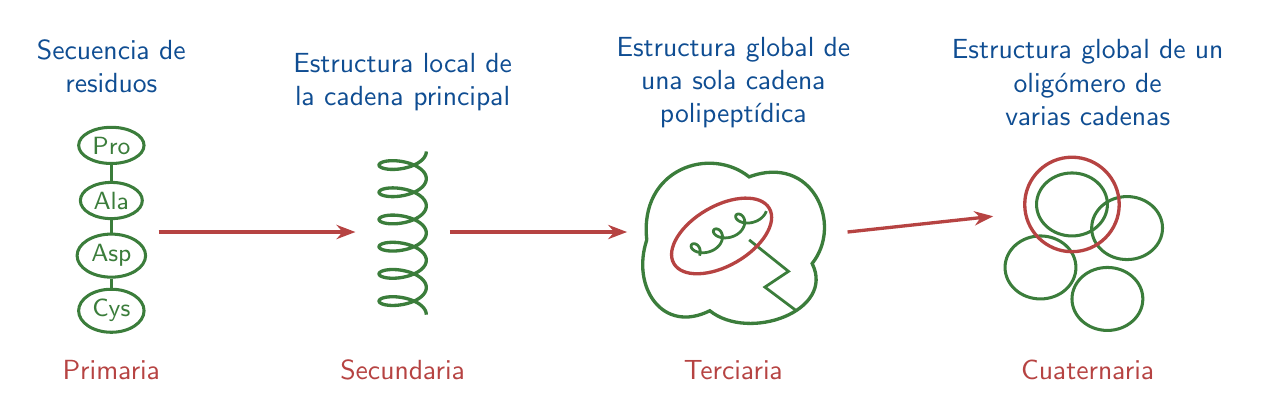
\begin{tikzpicture}[font=\normalsize]
  % ---- Primaria: secuencia de residuos
  \node[anotacion, align=center] at (0,2.6) {Secuencia de\\residuos};
  \foreach \r/\y in {Pro/1.6, Ala/0.9, Asp/0.2, Cys/-0.5} {
    \node[draw=apVerde, ellipse, line width=1.1pt, inner sep=1.5pt, font=\small, apVerde] (\r) at (0,\y) {\r};
  }
  \draw[apVerde, line width=1.1pt] (Pro) -- (Ala) (Ala) -- (Asp) (Asp) -- (Cys);
  \node[apRojo] at (0,-1.25) {Primaria};

  % ---- Secundaria: hélice (muelle visto de lado)
  \node[anotacion, align=center] at (3.7,2.4) {Estructura local de\\la cadena principal};
  \draw[apVerde, line width=1.2pt, domain=0:12*pi, samples=400, smooth, variable=\t]
    plot ({3.7+0.3*cos(\t r)}, {-0.55+0.055*\t+0.13*sin(\t r)});
  \node[apRojo] at (3.7,-1.25) {Secundaria};

  % ---- Terciaria: plegamiento global con una hélice rodeada
  \node[anotacion, align=center] at (7.9,2.4) {Estructura global de\\una sola cadena\\polipeptídica};
  \draw[apVerde, line width=1.2pt]
    (6.8,0.4) .. controls (6.7,1.3) and (7.6,1.6) .. (8.1,1.2) .. controls (8.9,1.5) and (9.3,0.6) .. (8.9,0.1)
              .. controls (9.2,-0.5) and (8.1,-0.9) .. (7.6,-0.5) .. controls (7.0,-0.8) and (6.6,-0.2) .. (6.8,0.4);
  \draw[apVerde, line width=1pt, domain=0:6*pi, samples=200, smooth, variable=\t]
    plot ({7.35+0.045*\t+0.12*cos(\t r)}, {0.2+0.03*\t+0.1*sin(\t r)});
  \draw[apVerde, line width=1pt] (8.1,0.4) -- (8.6,0.0) -- (8.3,-0.2) -- (8.7,-0.5);
  \draw[apRojo, line width=1.2pt, rotate around={30:(7.75,0.45)}] (7.75,0.45) ellipse (0.7 and 0.38);
  \node[apRojo] at (7.9,-1.25) {Terciaria};

  % ---- Cuaternaria: oligómero de varias cadenas
  \node[anotacion, align=center] at (12.4,2.4) {Estructura global de un\\oligómero de\\varias cadenas};
  \foreach \cx/\cy in {12.2/0.85, 11.8/0.05, 12.65/-0.35, 12.9/0.55} {
    \draw[apVerde, line width=1.1pt] (\cx,\cy) circle [x radius=0.45, y radius=0.4];
  }
  \draw[apRojo, line width=1.2pt] (12.2,0.85) circle (0.6);
  \node[apRojo] at (12.4,-1.25) {Cuaternaria};

  % ---- flechas entre niveles
  \draw[->, apRojo, line width=1.2pt] (0.6,0.5) -- (3.1,0.5);
  \draw[->, apRojo, line width=1.2pt] (4.3,0.5) -- (6.55,0.5);
  \draw[->, apRojo, line width=1.2pt] (9.35,0.5) -- (11.2,0.7);
\end{tikzpicture}
% ---------------------------
\end{document}
